\chapter{Background} \label{Background}

Machine Learning (ML) is a programming approach for creating Artificial Intelligence (AI) systems in non-trivial environments by making use of experiences and a substantial amount of data \cite{ml, Goodfellow-et-al-2016, russell2016artificial, lecun2015deep}. 

One of the most trivial Machine Learning examples is classifying handwritten digits by making use of the MNIST database \cite{mnist}. It is conspicuous that Machine Learning is the only viable option in developing this kind of applications as it is tough (if not impossible) to come up with hard-coded rules for each class case \cite{Goodfellow-et-al-2016}.

\textbf{Notation.} We will follow the same mathematic conventions used in \cite{Goodfellow-et-al-2016} (See Table \ref{tab: notations}).

% \begin{itemize}
%     \item $x$ - A scalar 
%     \item $\boldsymbol{x}$ - A vector 
%     \item $\boldsymbol{M}$ - A matrix 
%     \item $\boldsymbol{M}^T$ - A transposed matrix
%     \item $x_{i}$ - Element $i$ from vector % $\boldsymbol{x}$, starting from 0
%     \item $\boldsymbol{X}_{i}$ - Row $i$ of matrix % $X$
%     \item $X_{i, j}$ - The element with row $i$ and % column $j$ from matrix $X$
%     \item $\boldsymbol{x} * \boldsymbol{y}$ - An % element-wise vector product
% \end{itemize}

\begin{table}[h!]
    \centering
    \begin{tabular}{l l}
        $x$ & A scalar \\
        $\boldsymbol{x}$ & A vector \\
        $\boldsymbol{M}$ & A matrix \\
        $\boldsymbol{M}^T$ & A transposed matrix \\
        $x_{i}$ & Element $i$ from vector $\boldsymbol{x}$, starting from 0 \\
        $\boldsymbol{X_{i}}$/$\boldsymbol{x_{i}}$ & Row $i$ of matrix $\boldsymbol{X}$ \\
        $X_{i, j}$ & The element with row $i$ and column $j$ from matrix $\boldsymbol{X}$ \\
        $\boldsymbol{x} * \boldsymbol{y}$ & An element-wise vector product \\
        $x^{(l)}$/$\boldsymbol{x^{(l)}}$/$\boldsymbol{X^{(l)}}$ & Depends on the context of $l$ \\
    \end{tabular}
    \caption{Notations \cite{Goodfellow-et-al-2016}}
    \label{tab: notations}
\end{table}

The aim of Machine Learning methods is to find a pattern in the features of data $\boldsymbol{X} \in \mathbb{R}^{n \times m}$, where $n$ is the number of data examples and $m$ is the number of features. Machine Learning can be classified into two major categories: supervised and unsupervised, but we are going to focus on supervised ML. Supervised ML operates on data that has been labelled with $\boldsymbol{y} \in \mathbb{R}^{n}$, where each $y_i$ corresponds to a row in $\boldsymbol{X}$, $f(\boldsymbol{x_i}) = y_i$, $f \colon \mathbb{R}^m \xrightarrow{} \mathbb{R}$. Our goal is to find a function $h \colon \mathbb{R}^m \xrightarrow{} \mathbb{R}$ which approximates $f$, $h(\boldsymbol{x_i}) \simeq f(\boldsymbol{x_i})$.

\section{Neural Networks}
(Feed-forward) Neural Networks (NN) \cite{ml, Goodfellow-et-al-2016, russell2016artificial, lecun2015deep} are a type of supervised Machine Learning inspired by real-world biological neurons. Each NN architecture is composed of artificial neurons.

\subsection{Artifical Neuron}

An artificial neuron \cite{ml, russell2016artificial, Goodfellow-et-al-2016} (See Figure \ref{fig:artificial_neuron}) has $m + 1$ inputs $x_{i \in \{0, ..., m\}}$ and $m + 1$ weights $w_{i \in \{0, ..., m\}}$, where input $0$ is a bias (we set $x_0 = 1$ so that $w_0$ becomes bias), with one output $y$. The neuron can be "activated" using an activation function $f$ such as sigmoid ($\sigma(x) = \frac{1}{1 + e^x}$), tanh ($tanh(x) = \frac{e^x - e ^{-x}}{e^x + e ^{-x}}$) or rectified linear unit (ReLU) ($f(x) = \begin{cases} 0, x < 0 \\ x, x \geq 0 \end{cases}$). The big picture is that the weights help the neuron learn a combination of inputs while the bias behaves like a learnable threshold. The idea behind the activation function is that we can define if a neuron is active or non-active based on the output value of $f$ (e.g. for sigmoid $f\colon \mathbb{R} \xrightarrow{} [0, 1]$, if $f < 0.5$ neuron is non-active).

$$y = f(z) = f(\sum_{i = 0}^{m} x_i \cdot w_i) = f(\boldsymbol{x}^T \boldsymbol{w}), x_0 = 1 \text{ and } w_0 \text{ bias}$$

\begin{figure}[h!]
  \centering
  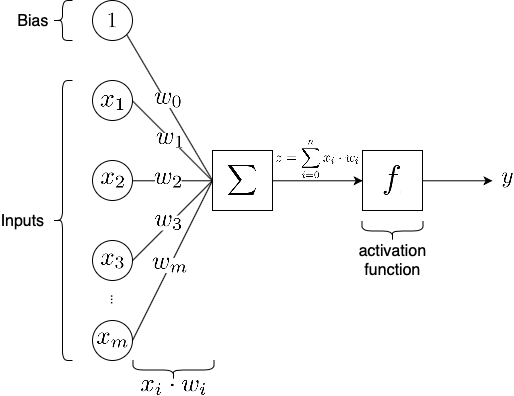
\includegraphics[scale=0.4]{images/artificial_neuron.png}
  \caption{Artificial neuron representation}
  \label{fig:artificial_neuron}
\end{figure}

\subsection{Neural Network Architecture}

We can then combine multiple artificial neurons to create a layered architecture (See Figure \ref{fig:nn}). There are 3 types of layers: the input layer, the output layer and the hidden layer. The input and output layers are mandatory and should match the number of neurons with the size of the input features and respectively output. The number of hidden layers, as well as, their number of neurons are part of the NN architecture, and they are referred to as the depth and respectively the width of the network \cite{ml, russell2016artificial, Goodfellow-et-al-2016}.

\begin{figure}[h!]
  \centering
  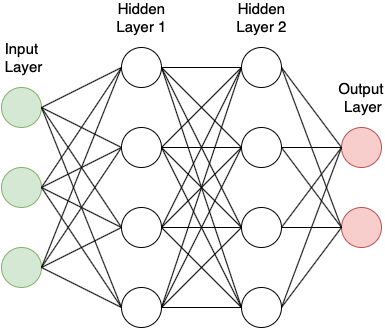
\includegraphics[scale=0.4]{images/nn.png}
  \caption{Neural network architecture with 2 hidden layers}
  \label{fig:nn}
\end{figure}

\subsection{Forward-propagation}

Each layer can be then written as $\boldsymbol{a^{(l)}} = f(\boldsymbol{z^{(l)}}) = f(\boldsymbol{W^{(l)}}^T \boldsymbol{a^{(l - 1)}})$, where
$\boldsymbol{a^{(l - 1)}} \in \mathbb{R}^{m + 1}$ is the input to layer $l$,
$\boldsymbol{a^{(l)}} \in \mathbb{R}^d$ is the output of layer $l$,
$\boldsymbol{W^{(l)}} \in \mathbb{R}^{(m + 1) \times d}$ are the weights associated with layer $l$, 
$a^{(l - 1)}_{0} = 1$ and
$\forall i.W^{(l)}_{i, 0}$ is bias. Therefore, each row $r$ in $\boldsymbol{W^{(l)}}$ corresponds to the weights associated with the $r$ neuron in layer $l$. $l = 0$ corresponds to the input layer and $l = L$ is the output layer. Now, we can write the whole architecture as following:

\begin{align*}
    \boldsymbol{y} &= \boldsymbol{a_{L}} \\
    \boldsymbol{a_{0}} &= \boldsymbol{x} \\
    \boldsymbol{a^{(l)}} &= f(\boldsymbol{W^{(l)}}^T \boldsymbol{a^{(l - 1)}}) \\
    \boldsymbol{y} &= f(\boldsymbol{W^{(L)}}^T f(\boldsymbol{W^{(L - 1)}}^T f(...f(\boldsymbol{W^{(0)}}^T \boldsymbol{x})))
\end{align*}

For now we can only (forward) propagate our input through the network and receive a random output, but we do not learn from our data $\boldsymbol{x}$ \cite{ml, russell2016artificial, Goodfellow-et-al-2016}.

\subsection{Back-propagation}

% The idea behind back-propagation is that when we are training the network, we would like to have a method for checking how good are we approximating the output against $\boldsymbol{y}$ and if we are not doing so great "learn" from it \cite{ml, russell2016artificial, Goodfellow-et-al-2016}.

Back-propagation \cite{ml, russell2016artificial, Goodfellow-et-al-2016} is a method in which we perform a backward pass through the network in order to adjust the weights of the neurons. The changing amount depends on how well we currently approximate the output against $\boldsymbol{y}$. If we have a bad approximation we adapt the weights in order to get closer to the true output.

We can develop a cost function $J$ that uses a loss function $L$ which will tell us how close are we to the actual solution. As an example, the least square error is a loss function used in regression $L(\boldsymbol{y^{(l)}}, \boldsymbol{a^{(l)}}) = \frac{1}{n} \sum^{n}_{i = 0} (y^{(l)}_i - a^{(l)}_i) ^ 2$, $J = L$. Our objective is to minimise the cost function $J$, as we would like to be as close as possible to the actual solution, while updating the weights (learn from our mistakes).

In order to update the weights correctly, we are going to use gradient descent (See Figure \ref{fig:learning_rate}), which is an iterative first-order method for finding a local minimum (or maximum as both problems are equivalent) or global minimum if the problem is convex. Therefore the update rule for our weights becomes:

\begin{align*}
    \boldsymbol{W^{(l)}} \gets \boldsymbol{W^{(l)}} - \alpha \frac{\partial J^{(l)}}{\partial \boldsymbol{W^{(l)}}}
\end{align*}

for each layer $l$, where $\alpha$ is the learning rate. The weights are updated starting from the output layer $l=L$ towards the input layer $l=0$ as when we update the layer $l=k$, we need the output of layer $l=k+1$ in order to compute $J^{(l)}$.

\subsection{Learning Rate}
The learning rate \cite{ml} $\alpha$ controls how much we change the weights. We have to be careful when setting the learning rate as if it is too low we might not reach the minimum (if we do not have enough iterations) or if it is too high, we are going to oscillate and might not find the minimum or even diverge (See Figure: \ref{fig:learning_rate}).

There are techniques that deal with this issue such as momentum or exact linear search optimisations for the learning rate: Golden Section or Newton-Raphson methods \cite{chong2013introduction}: 

$$\alpha^{(j)} \in \argmin{\alpha \geq 0} {\boldsymbol{W^{(l)}} - \alpha^{(j)} \frac{\partial J^{(l)}}{\partial \boldsymbol{W^{(l)}}}}\textrm{, for each iteration j}$$

\begin{figure}[]
  \centering
  \begin{subfigure}[b]{0.32\linewidth}
    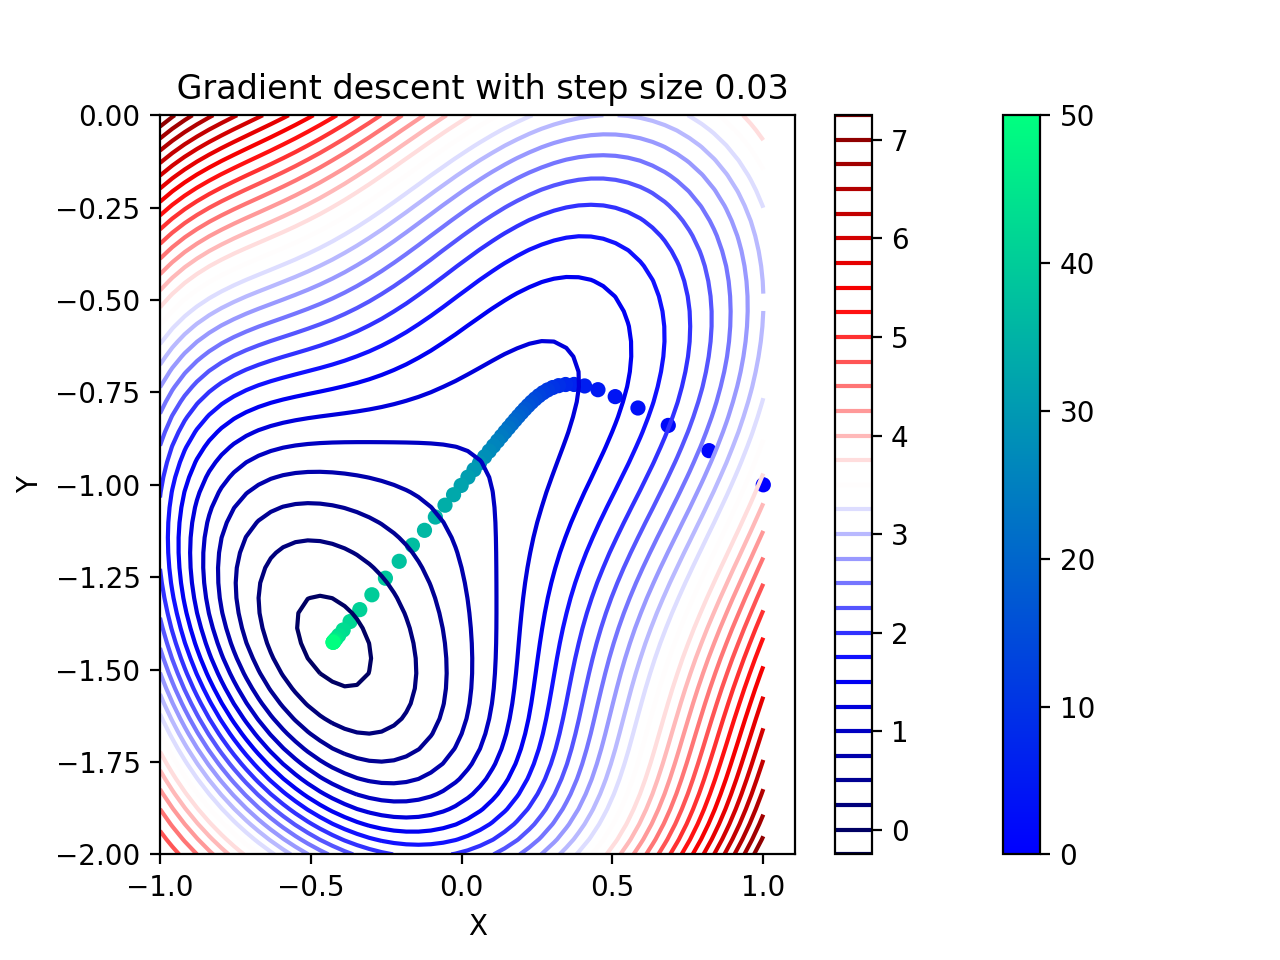
\includegraphics[width=\linewidth]{images/gradient_descent_just_right.png}
     \caption{Learning rate is just right}
  \end{subfigure}
  \begin{subfigure}[b]{0.32\linewidth}
    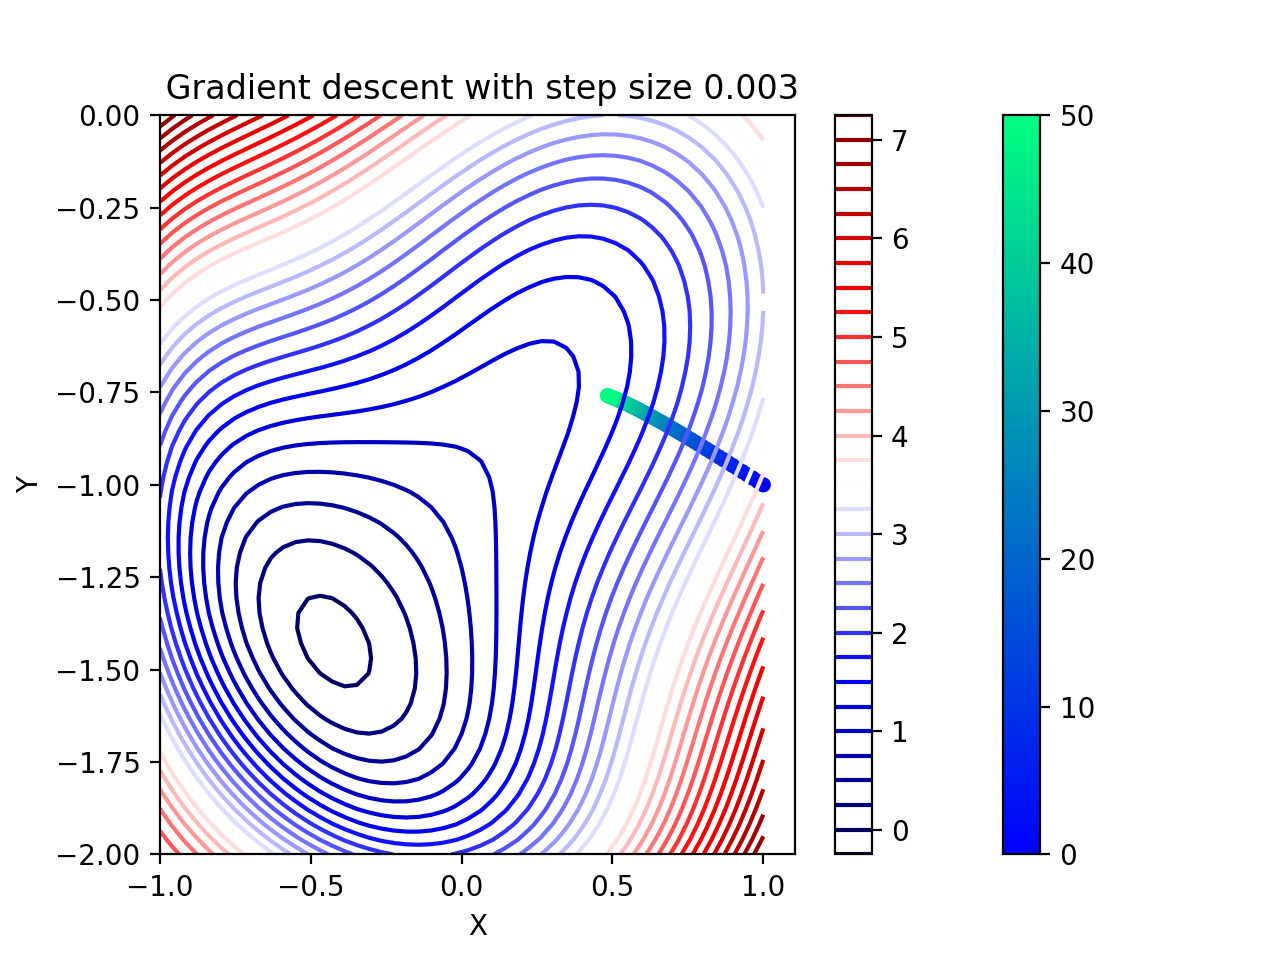
\includegraphics[width=\linewidth]{images/gradient_descent_too_small.png}
     \caption{Learning rate is too small}
  \end{subfigure}
  \begin{subfigure}[b]{0.32\linewidth}
    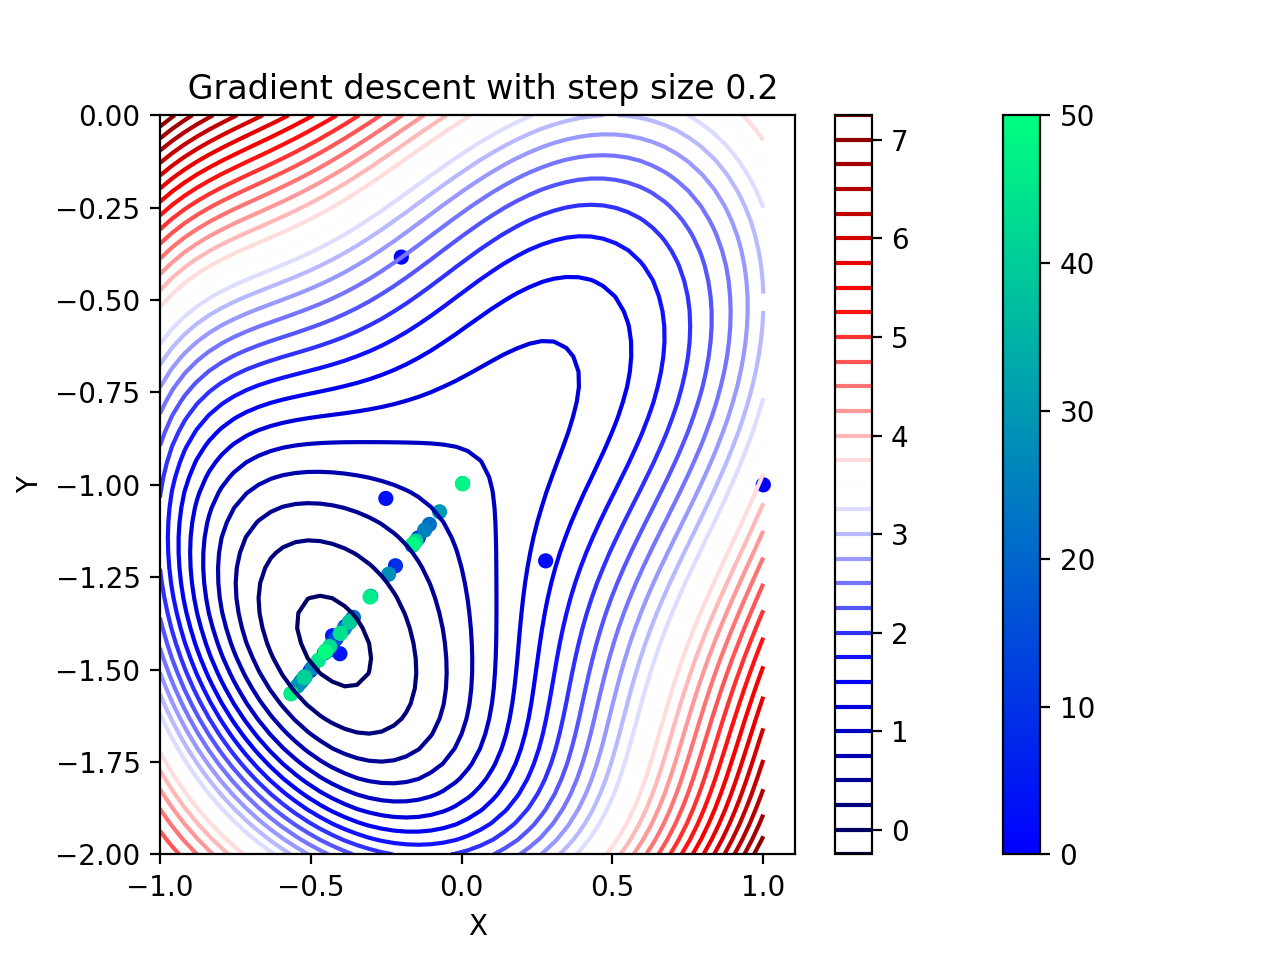
\includegraphics[width=\linewidth]{images/gradient_descent_too_high.png}
     \caption{Learning rate is too high}
  \end{subfigure}
  \caption{Gradient descent with a reasonable, too small or too high learning rate. When the learning rate is reasonable we reach a minimum point, when the learning rate is too small we do not reach a minimum if the number of iterations is not high enough, and when the learning rate is too high we start to oscillate and might even diverge}
  \label{fig:learning_rate}
\end{figure}
\subsection{Training}
Putting it altogether, in order to train the Neural Network, for each training example $\boldsymbol{x_i}$ we:
\begin{itemize}
    \item execute a forward propagation to get $\forall l \in \{0, ..., L\}.\boldsymbol{a^{(l)}}$
    
    \item back-propagate to update the weights $\forall l \in \{0, ..., L\}.\boldsymbol{W^{(l)}}$ following the gradient descent formula
\end{itemize}

However, before training the model, we have to process the data so that we have a mechanism of improving (by tuning the hyper-parameters) and evaluating the model. There are multiple ways of splitting the data, but we are going to focus on the most important ones: holdout and $k$-fold cross validation \cite{ml, russell2016artificial, Goodfellow-et-al-2016}.

The holdout method is mostly used when there is a lot of training data. The training data is split into three subsets: training, validation and testing (usually 60\% training, 20\% validation, 20\% testing). The model is then trained on the training data and evaluated on the validation data in order to improve the performance of the network by tuning the model hyper-parameters. The process of passing the entire training and validation data through the model is known as an epoch. The process can then be repeated $n$ epochs until no further improvement is noticed or over-fitting occurs. When the model is tuned, we run a final evaluation on the testing data to report the final results of our model. We do not tune the model on the testing data as this would contradict our generalisation assumption and will make the evaluation redundant.

In the case of having low amounts of training data, we can opt for the $k$-fold cross validation method. The idea behind this method is that we are going to partition our data set into two groups: training and testing $k$ times. The partitioning is achieved as seen in Figure \ref{fig:cross_fold}. The training process is similar to the holdout method, but the evaluation results are averaged over the splits. It is worth mentioning that there are many variants to this method such as: leave $n$ out, leave one out, $k$-fold cross validation with validation and test set and many more.

\begin{figure}[h!]
  \centering
  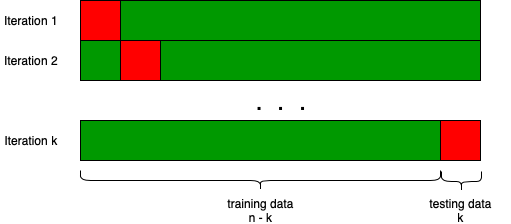
\includegraphics[scale=0.5]{images/cross_fold.png}
  \caption{$k$-fold cross validation. Training data is represented with green and testing data is represented with red}
  \label{fig:cross_fold}
\end{figure}


\subsection{Evaluation}
At each evaluation step in our training pipeline, we can report a series of useful statistical measures such as loss over model complexity, precision, accuracy, recall, $F_1$ measure, confusion matrices and others \cite{ml, russell2016artificial, Goodfellow-et-al-2016}.

\subsection{Over-fitting}
Over-fitting \cite{ml, russell2016artificial, Goodfellow-et-al-2016} occurs when the model's predictions are almost perfectly matching the training data targets, meaning that it cannot generalise for unseen data. The opposite phenomenon is under-fitting and happens when the model is under-trained and cannot make any useful predictions. Formally, when the model under-performs, it has high bias, and when the model over-performs, it has high variance (See Figure \ref{fig:overfit}).

\begin{figure}[h!]
  \centering
  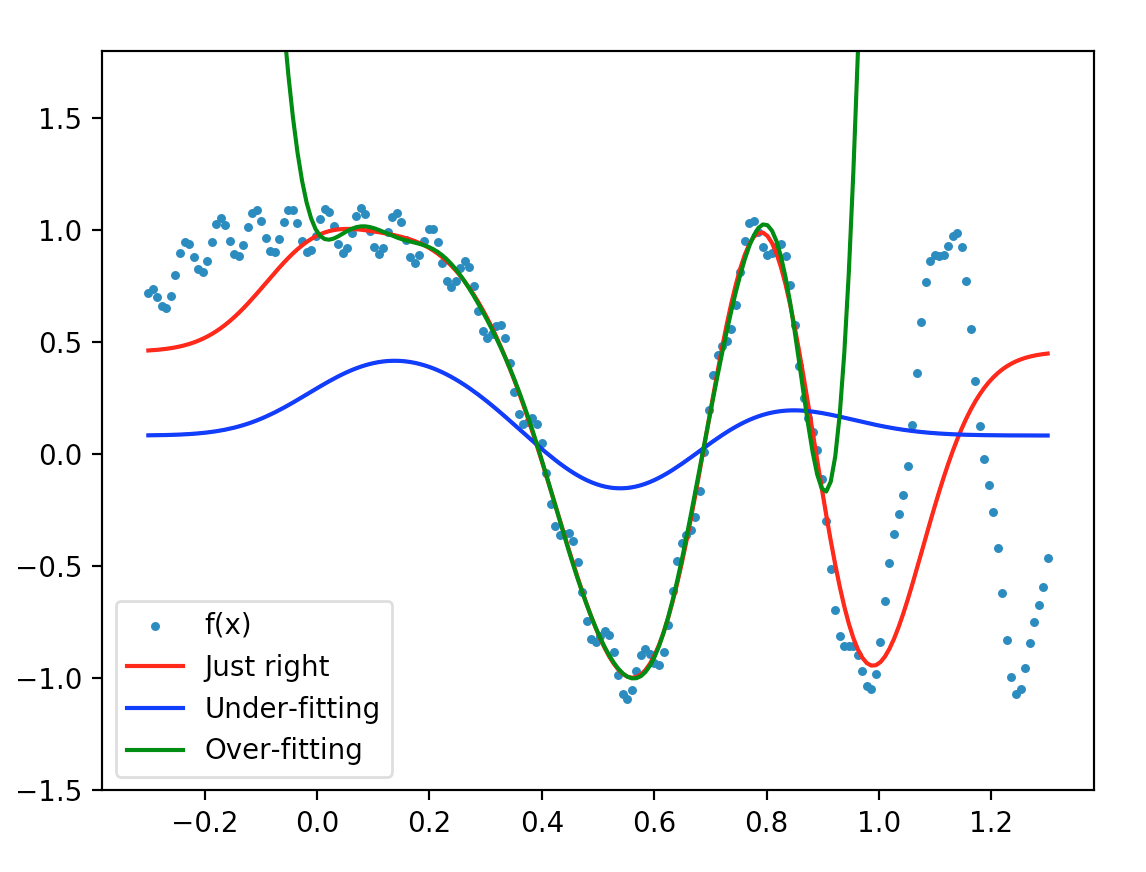
\includegraphics[scale=0.32]{images/overfit.png}
  \caption{Over-fitting example. Blue dots represent the actual function we are trying to approximate, the red function is just right, the green function is over-fitting, the blue function is under-fitting. The model was trained on the interval $[0, 0.9]$}
  \label{fig:overfit}
\end{figure}

Over-fitting starts at the point where the cost function starts increasing on the testing data, even though it keeps decreasing on the training data (See Figure \ref{fig:overfit_thresh}).

\begin{figure}[h!]
  \centering
  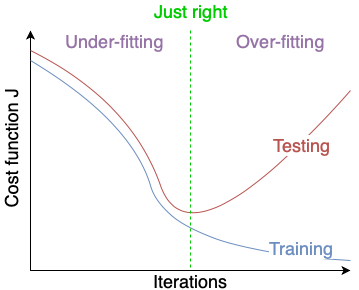
\includegraphics[scale=0.6]{images/overfit_tresh.png}
  \caption{Over-fitting threshold}
  \label{fig:overfit_thresh}
\end{figure}

\subsection{Regularisation}
To overcome the over-fitting problem we can use different approaches such as: early stopping (manually stop the training process when over-fitting is spotted), dropout (assign a probability that a neuron will "fire"), adding noise to data, L-norm regularisation (add a penalty term to the loss function; e.g. L1, L2, max norm) \cite{ml, russell2016artificial, Goodfellow-et-al-2016}.

L1 regularisation is used to "get rid" of weights by effectively setting them to 0. Intuitively, this means that we are going to only keep meaningful features.

$$J(\boldsymbol{W}) = L(\boldsymbol{y}, \boldsymbol{a}) + \lambda \sum_{w} |w|\textrm{, where $\lambda$ is the regularisation factor}$$

L2 regularisation is used to "punish" large weights, thus favouring small weights. This means that our $h$ will not oscillate that much due to high weights. It should be noted that L2 is more sensible to outliers than L1.

$$J(\boldsymbol{W}) = L(\boldsymbol{y}, \boldsymbol{a}) + \lambda \sum_{w} w^2\textrm{, where $\lambda$ is the regularisation factor}$$

\section{Recurrent Neural Networks}
Neural Networks are great for solving regression, logistic and classifying problems, but they do not handle well time-series problems. One of the reasons why is that time-series problems depend on the previous state and due to the acyclic graph design of the NN architecture, this information cannot be propagated through the network, and it is lost.

Recurrent Neural Networks (RNN) \cite{ml, LSTM_blog} are tackling this sort of issue by introducing a backwards edge from the last hidden layer to the first hidden layer in the NN architecture that carries the previous state information. Thus, if we unfold the RNN architecture, we can notice that each previous outcome is connected to the current one (See Figure \ref{fig:RNN}).

\begin{figure}[h]
  \centering
  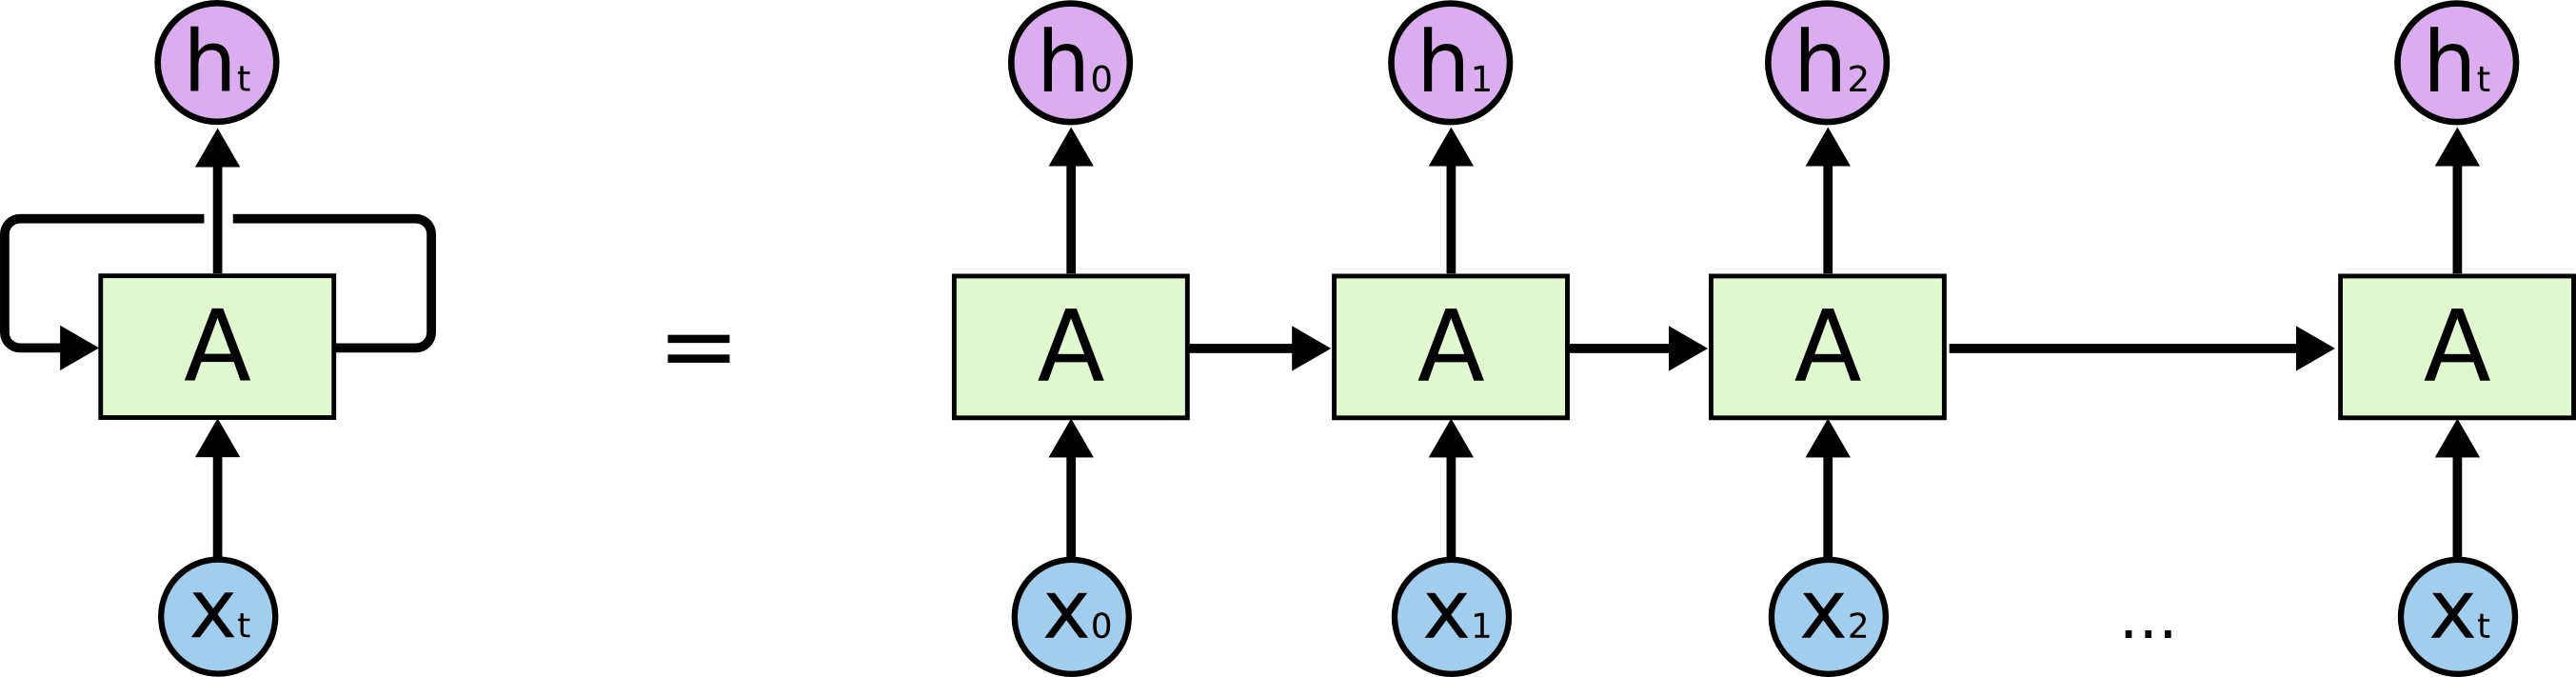
\includegraphics[scale=0.30]{images/RNN-unrolled.png}
  \caption{Recurrent Neural Network \cite{LSTM_blog}}
  \label{fig:RNN}
\end{figure}

One of the major issues with RNNs is that they do not train well. They use back-propagation through time, which is a similar training process to the NN one, but it achieved over the length of the time series. This procedure suffers from the vanishing or exploding gradient problem. The vanishing gradient problem states that if the gradient of the weights is less than 1 at time $t$, than as $t \xrightarrow{} 0$ so is $\nabla w^{(t)} \xrightarrow{} 0$. In the case of the weights being matrices, we use the L2 norm $\left\lVert \nabla \boldsymbol{W^{(t)}} \right\rVert = \sqrt{\lambda}$, where $\lambda$ is the largest eigenvalue of $\boldsymbol{W^{(t)}}$. The exploding gradient problem states that if the gradient of the weights is greater than 1 at time $t$, than as $t \xrightarrow{} 0$, $\nabla w^{(t)} \xrightarrow{} \infty$ (analogue for $\boldsymbol{W^{(t)}}$). Therefore, only the first layers from the back are trained properly if the time-series length is even remotely big. A common solution (but not preferred) to this problem is to change the architecture by adding extra backward edges between hidden layers so that we can propagate the gradient more efficiently.

\section{Long Short-Term Memory (LSTM)}
The Long Short-Term Memory (LSTM) \cite{hochreiter1997long, LSTM_blog} is a type of Recurrent Neural Network that solves the vanishing and exploding gradient problem by adding internal gates to the architecture to control the gradient flow during training.

As seen in Figure \ref{fig:LSTM}, the LSTM cell contains four types of internal gates that control the flow of information, and three types of input: $\boldsymbol{x^{(t)}}$ (the actual input at time $t$), $\boldsymbol{c^{(t)}}$ (cell state at time $t$, which we do not expose outside the internal architecture) and $\boldsymbol{h^{(t)}}$ (hidden state at time $t$).

\begin{figure}[h]
  \centering
  \begin{subfigure}[b]{0.6\linewidth}
    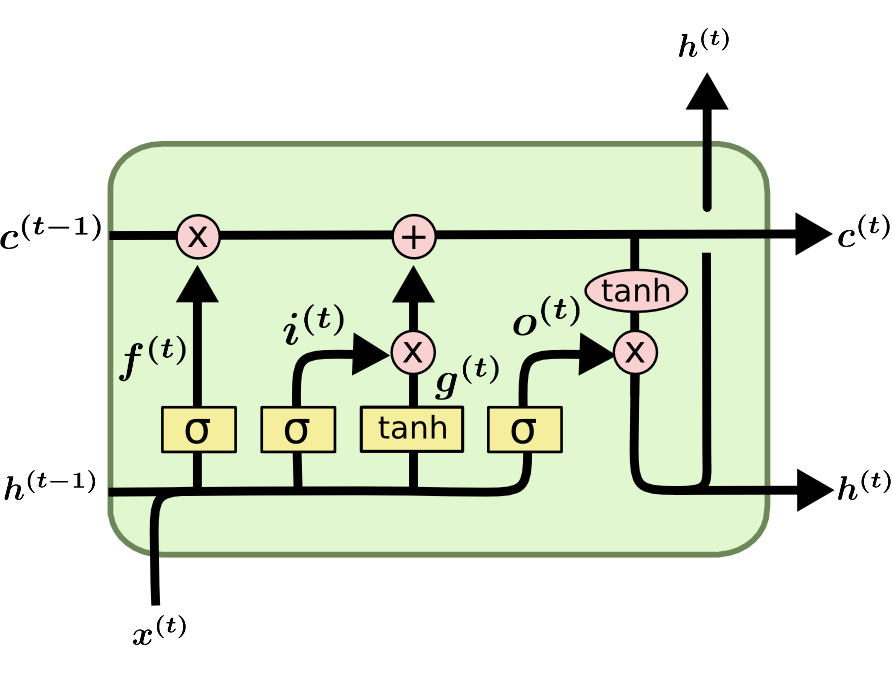
\includegraphics[width=\linewidth]{images/lstm_archi_cell.png}
  \end{subfigure}
  \hfill
  \begin{subfigure}[b]{0.6\linewidth}
    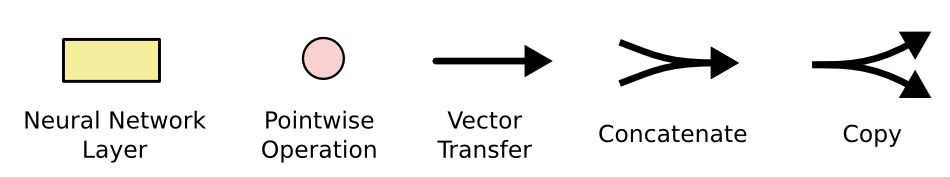
\includegraphics[width=\linewidth]{images/LSTM2-notation.png}
  \end{subfigure}
  \caption{LSTM cell \cite{LSTM_blog}}
  \label{fig:LSTM}
\end{figure}

The \textbf{forget} gate $\boldsymbol{f^{(t)}} = \sigma(\boldsymbol{W^{(f)}} \cdot [\boldsymbol{h^{(t - 1)}}, \boldsymbol{x^{(t)}}] + \boldsymbol{b^{(f)}})$, where $\sigma$ is the sigmoid function, $\boldsymbol{W^{(f)}}$ are the weights and $\boldsymbol{b^{(f)}}$ is the bias associated with the \textbf{forget} gate, controls the amount of information that we would like to forget as $\boldsymbol{f^{(t)}} \colon \mathbb{R}^n \xrightarrow{} [0, 1]$, so when $\boldsymbol{f^{(t)}}$ tends to 0 we forget more about the previous states.

The \textbf{input} gate $\boldsymbol{i^{(t)}} = \sigma(\boldsymbol{W^{(i)}} \cdot [\boldsymbol{h^{(t - 1)}}, \boldsymbol{x^{(t)}}] + \boldsymbol{b^{(i)}})$ controls how much information we would like to keep from the input. As in the case of the \textbf{forget} gate, when $\boldsymbol{i^{(t)}}$ tends to 0 we discard more information.

The \textbf{gate} gate $\boldsymbol{g^{(t)}} = tanh(\boldsymbol{W^{(g)}} \cdot [\boldsymbol{h^{(t - 1)}}, \boldsymbol{x^{(t)}}] + \boldsymbol{b^{(g)}}$ decides the importance of the data. Because $\boldsymbol{g^{(t)}}\colon \mathbb{R}^n \xrightarrow{} [-1, 1]$, if $\boldsymbol{g^{(t)}}$ tends to 1 we consider the input to be more important.

The next cell state is given by $\boldsymbol{c^{(t)}} = \boldsymbol{f^{(t)}} * \boldsymbol{c^{(t - 1)}} + \boldsymbol{i^{(t)}} * \boldsymbol{g^{(t)}}$. The cell state combines the output of all internal gates and contains the information that should be carried to the next state.

The \textbf{output} gate $\boldsymbol{o^{(t)}} = \sigma(\boldsymbol{W^{(o)}} \cdot [\boldsymbol{h^{(t - 1)}}, \boldsymbol{x^{(t)}}] + \boldsymbol{b^{(o)}})$ controls how much information we show to the user. As in the case of the \textbf{forget} and \textbf{input} gates, if $\boldsymbol{o^{(t)}}$ tends to 0 we output less information.

The actual output is given by the hidden state $\boldsymbol{h^{(t)}} = \boldsymbol{o^{(t)}} * tanh(\boldsymbol{c^{(t)}})$.

The particular design of this architecture solves the vanishing and exploding gradient problems by making use of the internal cell state $\boldsymbol{c^{(t)}}$. During training, the gradients flow more efficiently along the line defined between $\boldsymbol{c^{(t - 1)}}$  and $\boldsymbol{c^{(t)}}$. Moreover, it can be further extended by adding more LSTM layers by connecting the output at each time step from layer $n - 1$ to the input of layer $n$ to create a stacked architecture that has a similar effect to a Deep Neural Network.

It should be mentioned that there exist various LSTM architectures and extensions that attempt to improve the overall performance of the network such as: Gated Recurrent Units (GRUs), LSTMs with peephole connections and many more. Some of the extended architectures have reduced computational cost due to a lower complexity design (e.g. the GRU has a lower number of internal gates compared to the LSTM architecture), but, they still achieve similar or insignificantly better prediction performance than LSTMs \cite{ml, russell2016artificial, Goodfellow-et-al-2016, hochreiter1997long, LSTM_blog}.